\documentclass[11pt,a4paper]{article}
\usepackage[margin=18mm,top=17mm,bottom=19mm]{geometry}
\usepackage{amsmath,amssymb,graphicx,array,fancyhdr,lastpage,textcomp}
\usepackage{fontspec}
\setmainfont{texgyreheros-regular.otf}[BoldFont=texgyreheros-bold.otf,ItalicFont=texgyreheros-italic.otf,BoldItalicFont=texgyreheros-bolditalic.otf]
\setlength{\parindent}{0pt}
\setlength{\parskip}{3pt}
\pagestyle{fancy}\fancyhf{}
\renewcommand{\headrulewidth}{0pt}\renewcommand{\footrulewidth}{0.3pt}
\fancyfoot[L]{\footnotesize by paper.shrit.in\quad |\quad normal}
\fancyfoot[R]{\footnotesize Page \thepage\ of \pageref{LastPage}}
\newcommand{\question}[3]{\par\vspace{8pt}\noindent\begin{minipage}[t]{0.075\linewidth}\textbf{#1)}\end{minipage}\begin{minipage}[t]{0.855\linewidth}#3\end{minipage}\hfill\begin{minipage}[t]{0.055\linewidth}\raggedleft(#2)\end{minipage}\par}
\begin{document}
{\LARGE\bfseries Question Paper}\hfill {\small Registration No.: \rule{33mm}{0.3pt}}\par\vspace{8pt}
\begin{center}{\large\bfseries MANIPAL FORMAT | PRACTICE PAPER}\\[6pt]{\bfseries THIRD SEMESTER B.TECH. | MIDSEM PRACTICE}\\[4pt]{\bfseries DISCRETE MATHEMATICAL STRUCTURES [MAT 2101]}\\[4pt]{\small COMPUTER SCIENCE AND ENGINEERING}\\[3pt]{\small SET A: ENSEMBLE OF PAST-PAPER QUESTIONS}\end{center}
\textbf{Marks: 30}\hfill\textbf{Suggested duration: 90 minutes}\par\vspace{3pt}\hrule\vspace{5pt}
{\small\textbf{Answer all questions.} Questions 1--5 are MCQs worth 1 mark each. Select one correct option per MCQ. The remaining questions are theory questions worth 25 marks in total; show working and draw labelled diagrams where appropriate. Modules 1-3. Independent practice paper; not an official university examination.}\par
\medskip\textbf{Section A: Multiple-choice questions (5 marks)}\par
\question{1}{1}{Which pair of conditions defines a complement $b$ of $a$ in a Boolean algebra?\par (A) $a\lor b=0,\ a\land b=1$\par (B) $a\lor b=1,\ a\land b=0$\par (C) $a\lor b=a,\ a\land b=b$\par (D) $a=b$}
\question{2}{1}{How many complements does each element of a Boolean algebra have?\par (A) None\par (B) At least two\par (C) Infinitely many\par (D) Exactly one}
\question{3}{1}{Which expression equals $a\lor(\neg a\land b)$?\par (A) $a\lor b$\par (B) $a\land b$\par (C) $\neg a\lor b$\par (D) $a$}
\question{4}{1}{Which expression is in disjunctive normal form (a disjunction of conjunctions of literals)?\par (A) $(x\lor y)\land z$\par (B) $\neg(x\lor y)$\par (C) $(x\land y)\lor(\neg x\land z)$\par (D) $(x\lor y)\land(\neg x\lor z)$}
\question{5}{1}{Which expression is in conjunctive normal form (a conjunction of disjunctions of literals)?\par (A) $(x\land y)\lor z$\par (B) $(x\lor y)\land(\neg x\lor z)$\par (C) $\neg(x\land y)$\par (D) $(x\land y)\lor(\neg x\land z)$}
\newpage\textbf{Section B: Theory questions (25 marks)}\par
\question{6}{5}{Draw the Hasse diagram for A = \{1, 2, 3, 12, 18, 36\}, ordered by divisibility: a is related to b iff a divides b. Is it a lattice? Justify. List all antichains of length more than one.}
\question{7}{4}{How many ways are there to select a total of 15 items from three types, subject to these limits?\par Type A: 1 to 4 items; Type B: 3 to 7 items; Type C: 5 to 10 items.}
\question{8}{3}{Show that the number of partitions of n with no part smaller than 3 equals the number of partitions of n+3 whose three largest parts are consecutive integers.}
\question{9}{3}{Find the 75th permutation of the five marks 0, 1, 2, 3, 4 in Fike's order.}
\question{10}{3}{Show that if G is a regular self-complementary graph of order n, then n = 4t + 1 for some integer t.}
\question{11}{3}{If G has p vertices and minimum degree \(\delta\)(G) \(\ge\) (p - 1)/2, prove that G is connected.}
\question{12}{4}{Use Dijkstra's algorithm to find the shortest paths from v\(_{1}\) to every other vertex in the directed network below. Show the steps.\par\centering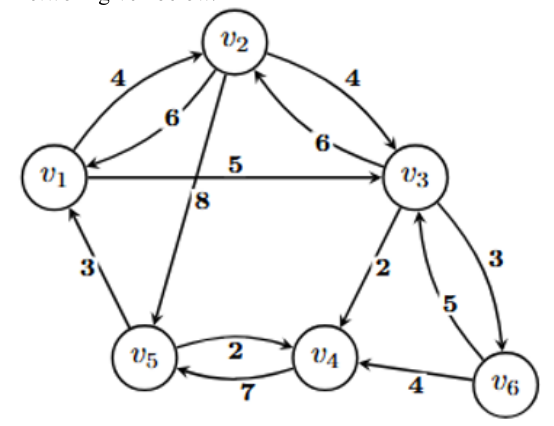
\includegraphics[width=0.64\linewidth]{dms-graph.png}}
\vfill\begin{center}\small End of question paper\end{center}\end{document}